\documentclass{Assignment}
\usepackage[utf8]{inputenc}
\usepackage[T1]{fontenc}
\usepackage{lmodern} % Optional, but recommended for better font rendering
\usepackage{subcaption}

% set the assignment number
\setassignmentnumber{1}
\setstartdate{02/08/2024}
\setenddate{07/08/2024}

% Add topics and authors before the \begin{document} command
% topics
\addtopic{On guarding the polygons with holes}
\addtopic{Art Gallery Problem with Rook and Queen sight}
\addtopic{Guards whose Range of Vision is 180$^{\circ}$}
\addtopic{A chromatic art gallery problem}
\addtopic{The Dispersive Art Gallery Problem}

% authors
\addauthor{Karthikeya - CS22B026}

% Add the name of the .bib file
\addbibresource{references.bib}

\begin{document}
\maketitlepage

% section for details of the problem set
\section*{Overview}
\printtopicsandauthors
\vspace{-0.8cm}
\subsection*{General Assumptions}
\vspace{-0.3cm}
\begin{itemize}
    \itemsep-0.3em
    \item \textbf{Polygon Type:} The polygon is simple, planar, has no holes and not curved.
    \item \textbf{Vertex Guards:} The guards are vertices and have a 360 degree field of view.
    \item \textbf{Stationary:} The guards are not allowed to move.
    \item \textbf{Infinite Visibility:} The guards have infinite visibility.
\end{itemize}
\vspace{-0.5cm}
\section*{On guarding the polygons with holes\supercite{on_guarding_polygons_with_holes}}
\begin{problem}[Problem Statement]
    For a given polygon $\mathcal{P}$ with $n$ vertices and $h$ holes, $\lfloor \frac{n+h}3 \rfloor$ vertex guards are always sufficient to guard the vertices of $\mathcal{P}$ and also the entire boundary.
\end{problem}
\vspace{-0.6cm}
\subsubsection*{Problem Specific Assumptions}
\vspace{-0.3cm}
\begin{itemize}
    \itemsep-0.3em
    \item \textbf{Existence of Holes:} The polygon $\mathcal{P}$ has $h$ holes. 
\end{itemize}
\vspace{-0.8cm}
\subsubsection*{State of the solution}
\vspace{-0.3cm}
\begin{itemize}
    \itemsep-0.3em
    \item The problem is solved for showing the sufficiency of $\lfloor \frac{n+h}3 \rfloor$ vertex guards for guarding the vertices of $\mathcal{P}$ and the entire boundary.
    \item The Shermer's conjecture still remains unsolved.
\end{itemize}
\vspace{-0.8cm}
\subsubsection*{Outline of the solution}
\vspace{-0.3cm}
\begin{itemize}
    \itemsep-0.3em
    \item They have used the idea of special triangulation to prove the results.
    \item They have shown that every polygon with holes has a special triangulation(See Fig \ref{fig:special_triangulation}).
    \item They have then used induction(See Fig \ref{fig:induction_step}) to show that $\lfloor \frac{n+h}3 \rfloor$ vertex guards are sufficient to guard the vertices.
    \begin{figure}[H]
        \centering
        \begin{minipage}{0.45\textwidth}
            \centering
            \begin{subfigure}[b]{\textwidth}
                \centering
                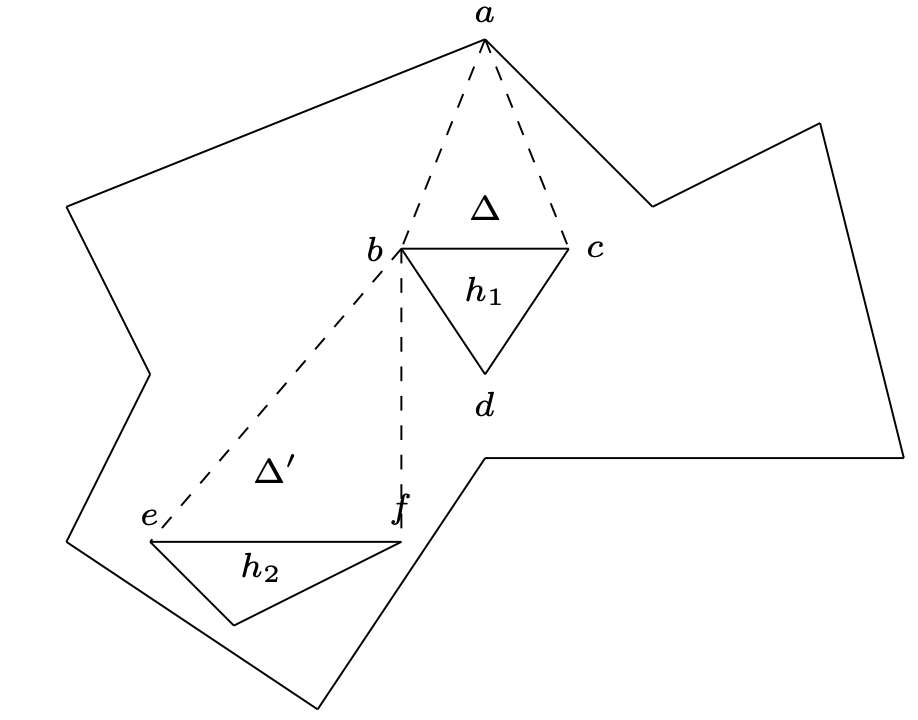
\includegraphics[width=0.9\textwidth]{images/special_triangulation.png}
                \caption{Special Triangulation}
                \label{fig:special_triangulation}
            \end{subfigure}
        \end{minipage}
        \hfill
        \begin{minipage}{0.45\textwidth}
            \centering
            \begin{subfigure}[b]{\textwidth}
                \centering
                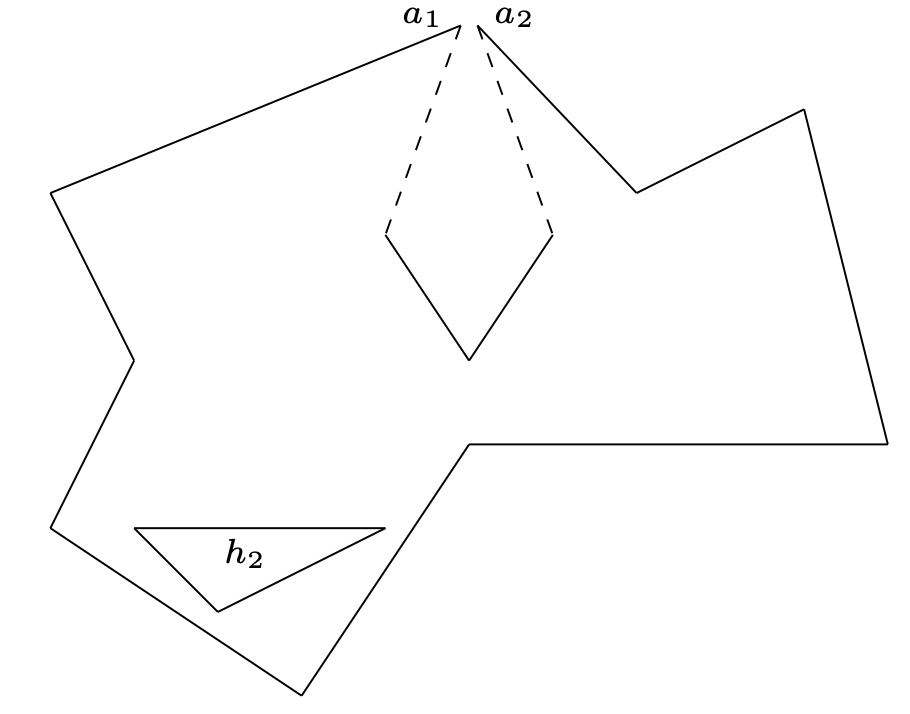
\includegraphics[width=0.9\textwidth]{images/induction_step.png}
                \caption{Induction Step}
                \label{fig:induction_step}
            \end{subfigure}
        \end{minipage}
        \caption{Images of Special Triangulation and Induction Step}
    \end{figure}
\end{itemize}
\vspace{-0.8cm}
\subsubsection*{Scope of further research}
\vspace{-0.3cm}
\begin{itemize}
    \itemsep-0.3em
    \item It would be interesting to see if the condition shown was necessary.
    \item It would be interesting to see if the Shermer's conjecture can be solved using the same approach.
\end{itemize}
\vspace{-0.7cm}
\section*{Art Gallery Problem with Rook and Queen sight\supercite{queen_and_rook_vision}}
\begin{problem}[Problem Statement]
    How many chess rooks or queens does it take to guard all the squares of a given polyomino?
\end{problem}
\vspace{-0.8cm}
\subsubsection*{Problem Specific Assumptions}
\vspace{-0.3cm}
\begin{itemize}
    \itemsep-0.3em
    \item \textbf{Queen and Rook Sight:} The guards have sight similar to that of a queen and a rook in chess.
    \item \textbf{Polygon Type:} The polygons considered are polyominoes. 
    \item \textbf{Polyomino Type:} The polyominoes are simple.
\end{itemize}
\vspace{-0.8cm}
\subsubsection*{State of the solution}
\vspace{-0.3cm}
\begin{itemize}
    \itemsep-0.3em
    \item It is shown that for a given polyomino with $n$ squares $\lfloor \frac n2 \rfloor$ rooks or $\lfloor \frac n3 \rfloor$ queens are sufficient and sometimes necessary.
    \item Finding the minimum number of rooks or queens required to guard a polyomino is $NP$-hard.
    \item The above results also apply for $d$ dimensional case. 
\end{itemize}
\vspace{-0.8cm}
\subsubsection*{Outline of the solution}
\vspace{-0.3cm}
\begin{itemize}
    \itemsep-0.3em
    \item They have first shown that $\lfloor \frac n2 \rfloor$ rooks are sometimes necessary for guarding a polyomino(See Fig \ref{fig:max_rook}).
    \item They have shown that $\lfloor \frac n3 \rfloor$ queens are sometimes necessary for guarding a polyomino(See Fig \ref{fig:max_queen}).
    \item They then proved that these are sufficient for guarding the polyomino and finding the optimal number is $NP$-hard.
    \begin{figure}[H]
        \centering
        \begin{minipage}{0.45\textwidth}
            \centering
            \begin{subfigure}[b]{\textwidth}
                \centering
                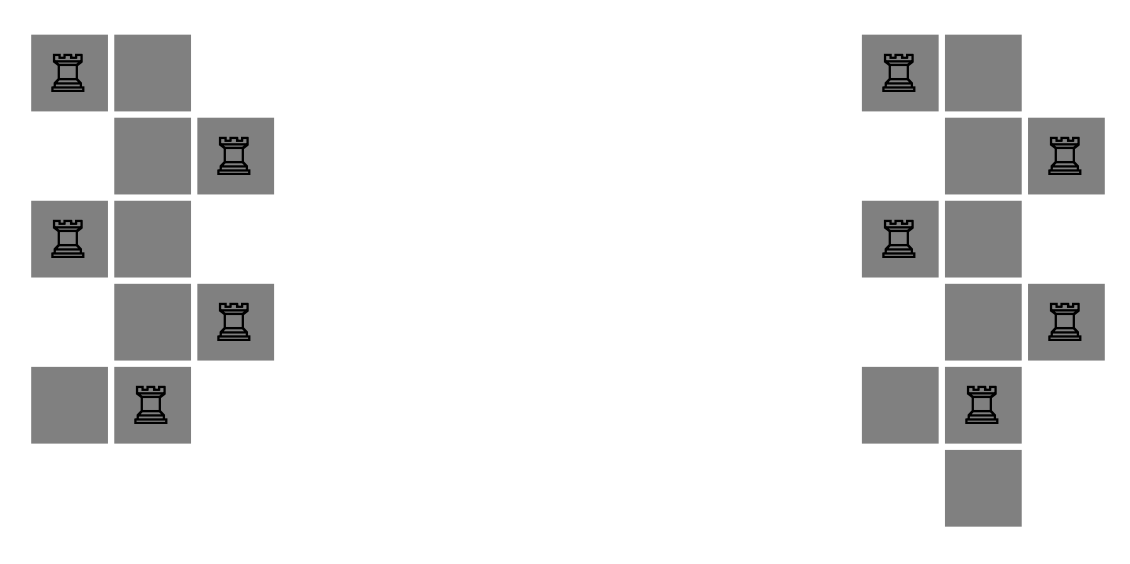
\includegraphics[width=\textwidth]{images/max_rook.png}
                \caption{Maximum Rook Polyomino}
                \label{fig:max_rook}
            \end{subfigure}
        \end{minipage}
        \hfill
        \begin{minipage}{0.45\textwidth}
            \centering
            \begin{subfigure}[b]{\textwidth}
                \centering
                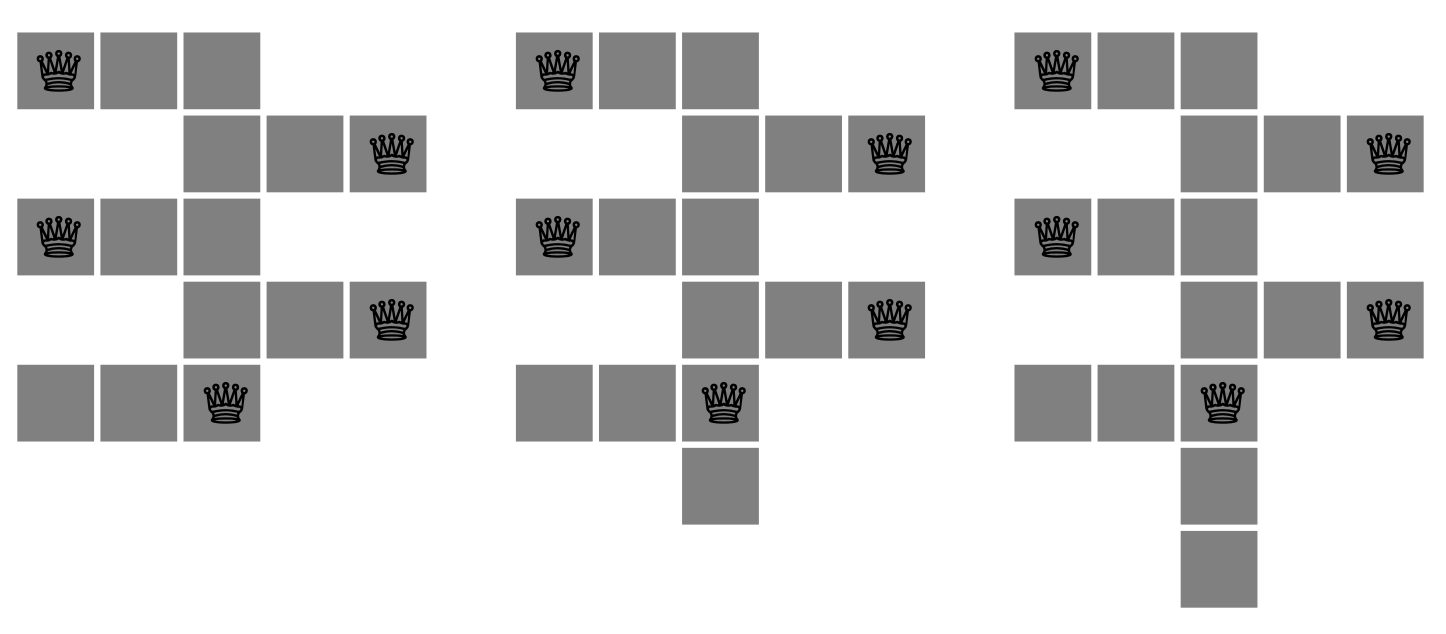
\includegraphics[width=\textwidth]{images/max_queen.png}
                \caption{Maximum Queen Polyomino}
                \label{fig:max_queen}
            \end{subfigure}
        \end{minipage}
        \caption{Polyominoes requiring maximum number of rooks and queens}
    \end{figure}
\end{itemize}
\vspace{-0.8cm}
\subsubsection*{Scope of further research}
\vspace{-0.3cm}
\begin{itemize}
    \itemsep-0.3em
    \item What are the kind of polyominoes that require the maximum number of rooks or queens?
    \item Would be interesting to see how many polyominoes require the maximum number of rooks or queens.
    \item Also there are 5 interesting open questions posed at the end of the paper.
\end{itemize}
\vspace{-0.7cm}
\section*{Guards whose Range of Vision is 180$^{\circ}$\supercite{180_guard_vision}}
\begin{problem}[Problem Statement]
    In any polygonal art gallery of $n$ sides it is possible to place $\lfloor \frac n3 \rfloor$ point guards whose range of vision is $180^{\circ}$ so that every interior point of the gallery can be seen by at least one guard.
\end{problem}
\vspace{-0.8cm}
\subsubsection*{Problem Specific Assumptions}
\vspace{-0.3cm}
\begin{itemize}
    \itemsep-0.3em
    \item {\bf 180$^\circ$ Sight:} The guards have a range of vision of $180^{\circ}$.
    \item {\bf Point Guards:} The guards can be placed anywhere in the polygon.
\end{itemize}
\vspace{-0.8cm}
\subsubsection*{State of the solution}
\vspace{-0.3cm}
\begin{itemize}
    \itemsep-0.3em
    \item The problem is solved, which also solved one of the open problems posed by Urrutia.
    \item The article also shows that $\lfloor \frac n3 \rfloor$ is the best possible upper bound for the problem.
\end{itemize}
\vspace{-0.8cm}
\subsubsection*{Outline of the solution}
\vspace{-0.3cm}
\begin{itemize}
    \itemsep-0.3em
    \item The proof is constructive in nature and naturally gives and $O(n^2)$ algorithm to find the guards.
    \item The proof is done by induction on cuts on the dual graph of a triangulation of the polygon.
    \item They have done exhaustive case analysis for the proof and have shown the results.
\end{itemize}
\vspace{-0.8cm}
\subsubsection*{Scope of further research}
\vspace{-0.3cm}
\begin{itemize}
    \itemsep-0.3em
    \item It would be interesting to see if the problem can be solved for polygons with holes.
    \item It would be interesting to see how the bounds of the problem change for human vision angle.
    \item It would be interesting if there exists an algorithm with better complexity than $O(n^2)$
\end{itemize}
\vspace{-0.7cm}
\section*{A chromatic art gallery problem\supercite{chromatic_art_gallery}}
\begin{problem}[Problem Statement]
    Suppose that two members of a finite point guard set $\mathcal{S} \subset \mathcal{P}$ must be given different colors if their visible regions overlap. What is the minimum number of colors required to color any guard set (not necessarily a minimal guard set) of a polygon $\mathcal{P}$ ? We call this number, $\chi_{G}(\mathcal{P})$, the chromatic guard number of $\mathcal{P}$.
\end{problem}
\vspace{-0.8cm}
\subsubsection*{Problem Specific Assumptions}
\vspace{-0.3cm}
\begin{itemize}
    \itemsep-0.3em
    \item {\bf Point Guards:} The guards are any point in the polygon.
\end{itemize}
\vspace{-0.8cm}
\subsubsection*{State of the solution}
\vspace{-0.3cm}
\begin{itemize}
    \itemsep-0.3em
    \item It was proved that for any spiral polygon $\mathcal{P}_{spi} \le 2$
    \item It was proved that for any staircase polygon $\mathcal{P}_{sta} \le 3$
    \item It was proved for any $k \in \mathbb{Z}^{+}$ there exists $ \mathcal{P}_k$ with $3k^2 + 2$ vertices such that $\chi_{G}(\mathcal{P}_k) \ge k$
\end{itemize}
\vspace{-0.8cm}
\subsubsection*{Outline of the solution}
\vspace{-0.3cm}
\begin{itemize}
    \itemsep-0.3em
    \item Figure \ref{fig:chromatic_lower_bound} shows the polygon $\mathcal{P}_k$ with $3k^2 + 2$ vertices such that $\chi_{G}(\mathcal{P}_k) \ge k$.
    \item The staircase polygons are solved by using the staircase polygons which are shown in Fig \ref{fig:staircase_polygon}.
    \item The spiral polygons are solved by using the reflex and convex subchains which are shown in Fig \ref{fig:spiral_polygon}.
    \begin{figure}[H]
        \centering
        \begin{minipage}{0.45\textwidth}
            \centering
            \vspace{-6.5cm}
            \begin{subfigure}[b]{\textwidth}
                \centering
                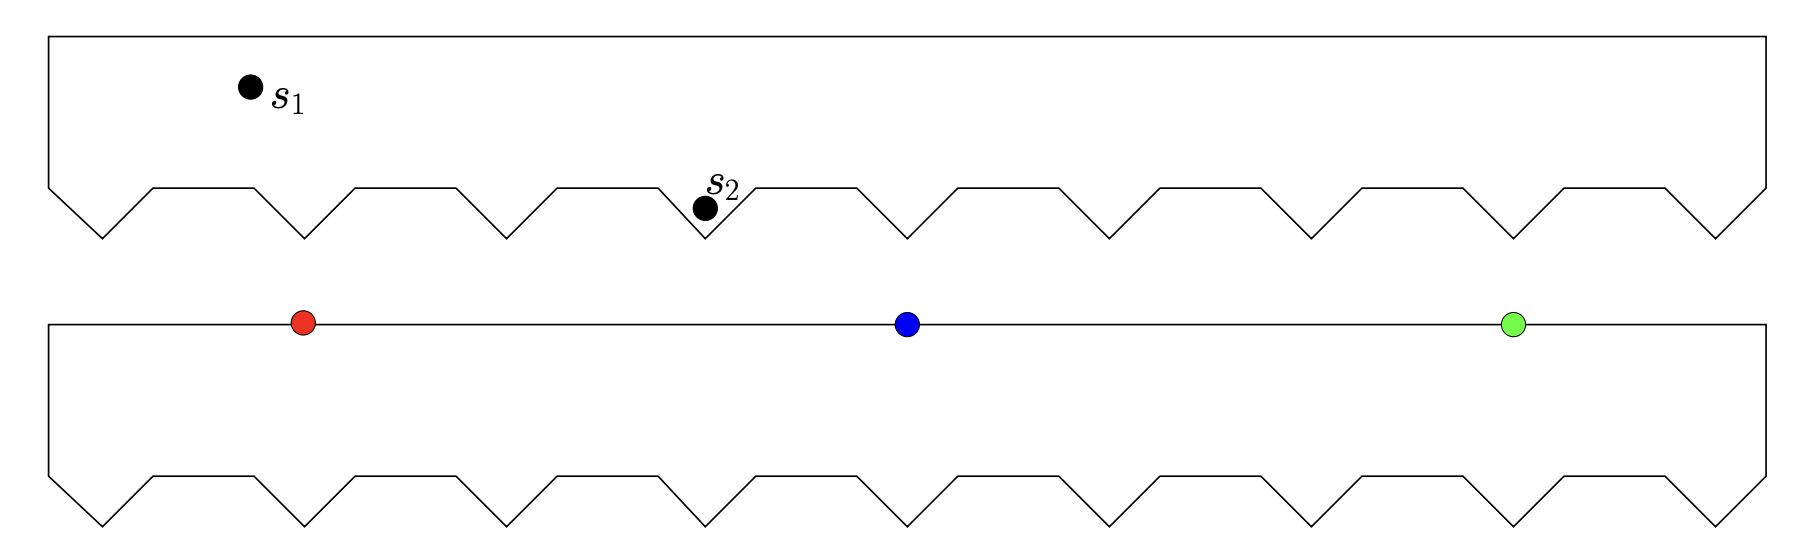
\includegraphics[width=0.9\textwidth]{images/lower_bound_chromatic.png}
                \caption{Polygon $\mathcal{P}_k$}
                \label{fig:chromatic_lower_bound}
            \end{subfigure}
            \vfill
            \begin{subfigure}[b]{\textwidth}
                \centering
                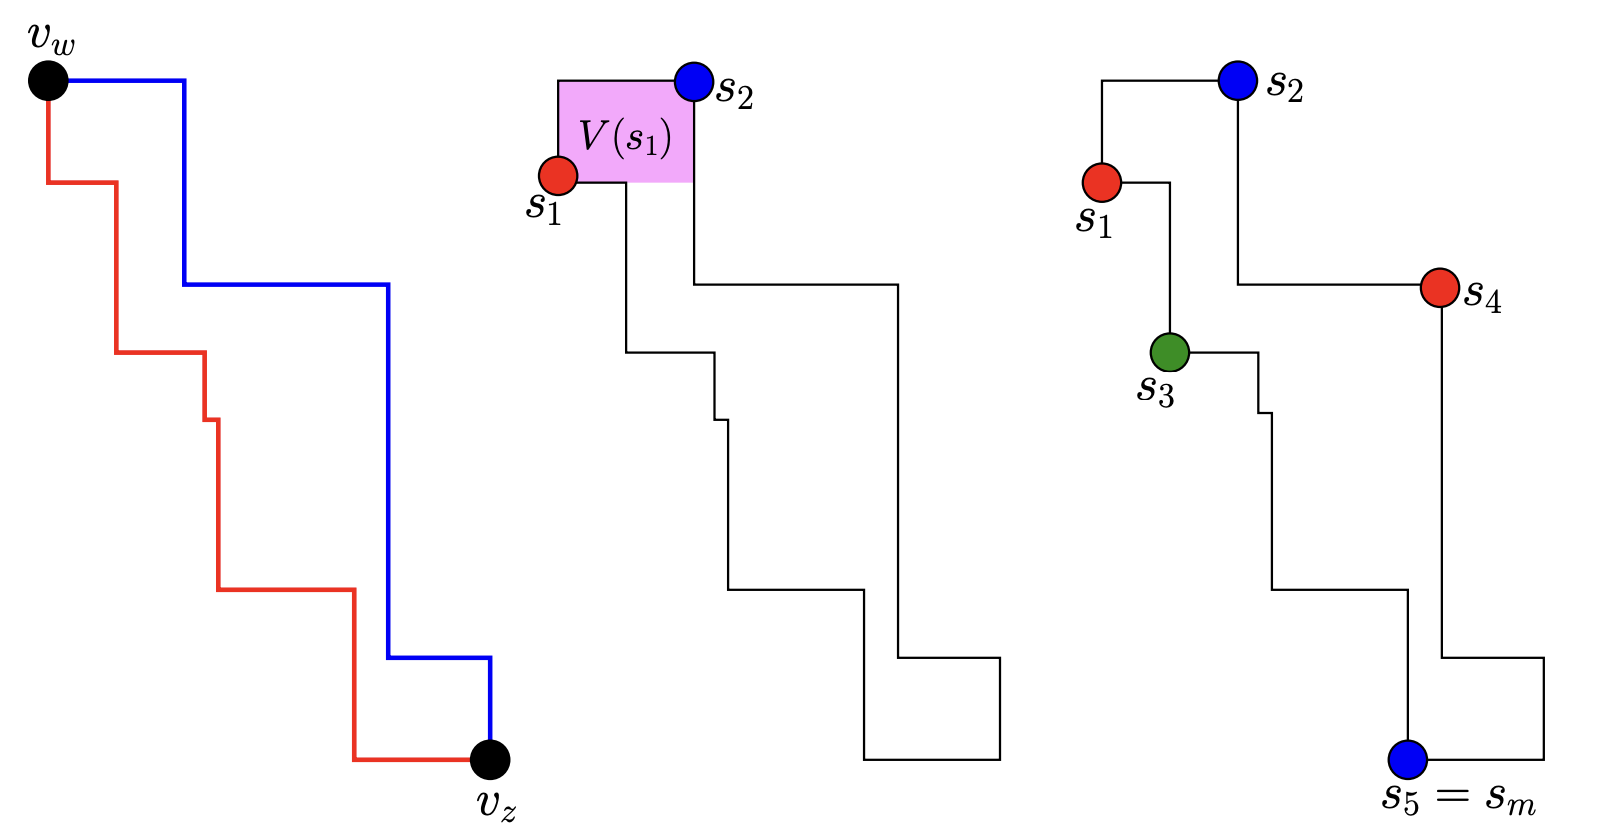
\includegraphics[width=0.9\textwidth]{images/staircase_polygon.png}
                \caption{Staircase Polygon}
                \label{fig:staircase_polygon}
            \end{subfigure}
        \end{minipage}
        \hfill
        \begin{minipage}[t]{0.45\textwidth}
            \centering
            \begin{subfigure}[b]{\textwidth}
                \centering
                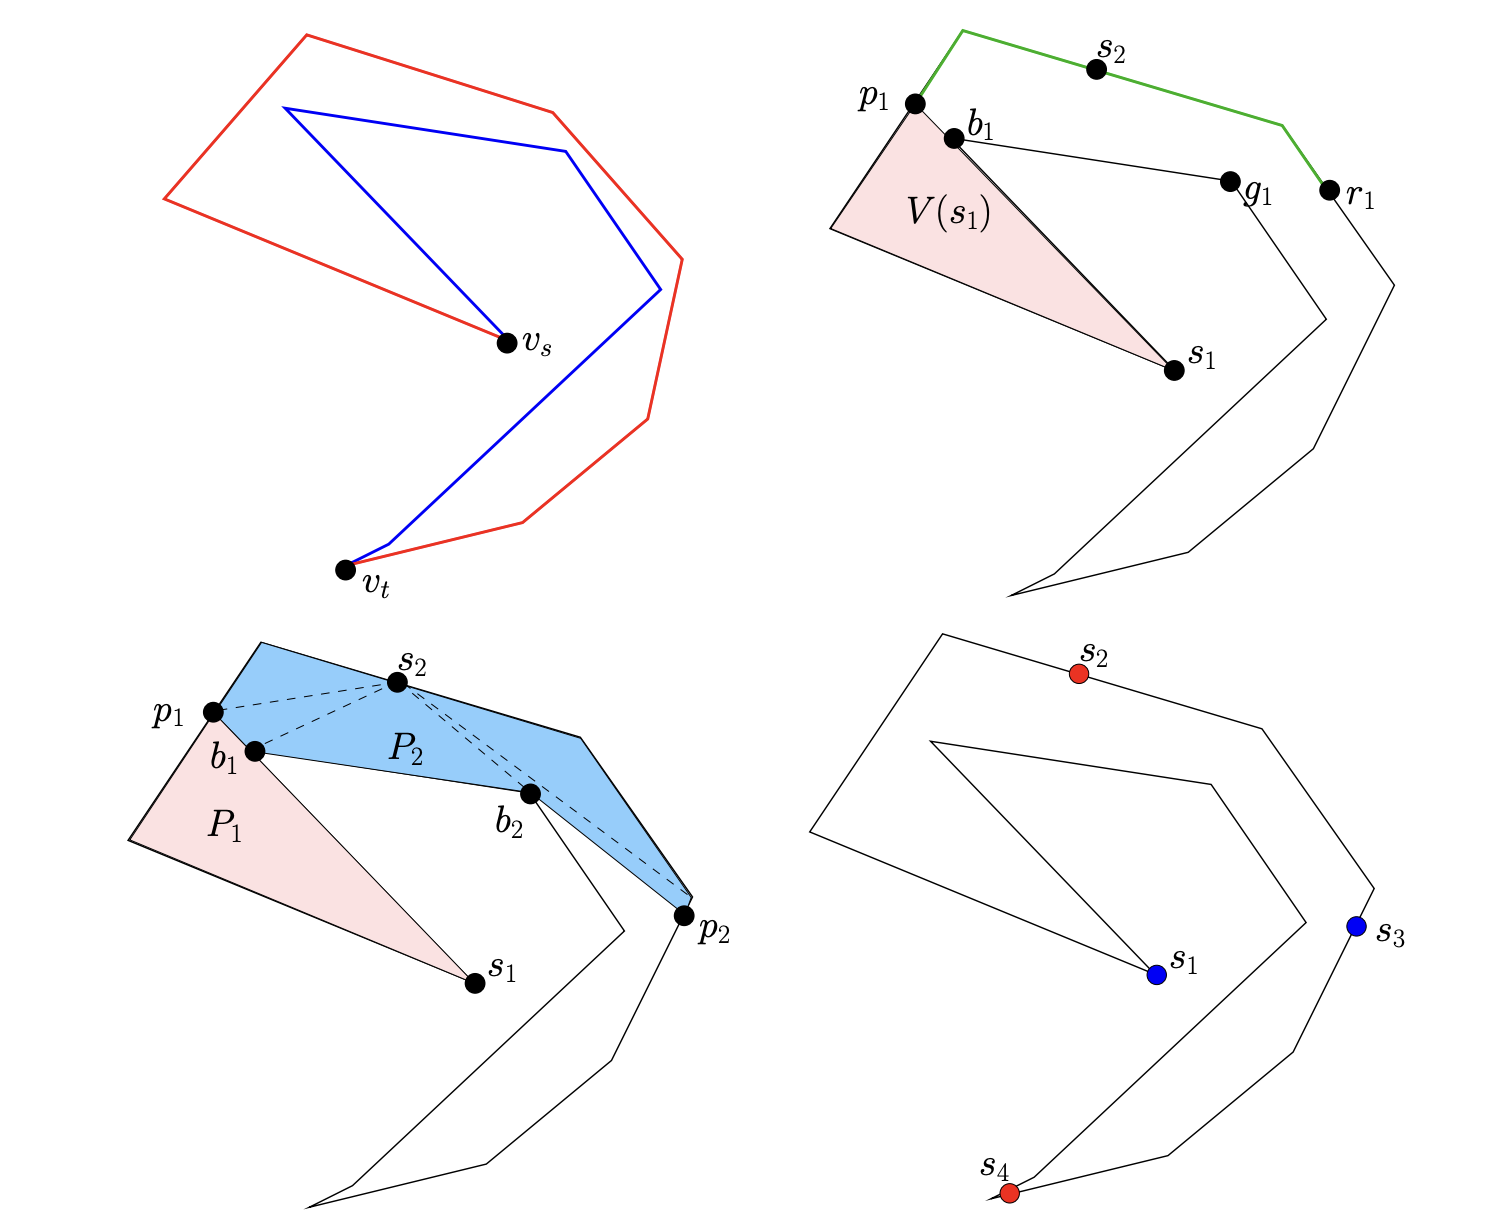
\includegraphics[width=0.9\textwidth]{images/spiral_polygon.png}
                \caption{Spiral Polygon}
                \label{fig:spiral_polygon}
            \end{subfigure}
        \end{minipage}
        \caption{Images of Key Polygons used in the paper}
    \end{figure}
\end{itemize}
\vspace{-0.8cm}
\subsubsection*{Scope of further research}
\vspace{-0.3cm}
\begin{itemize}
    \itemsep-0.3em
    \item It would be interesting to see if the problem can be solved for all orthogonal polygons.
    \item Finding a bound better than $\lfloor \frac n3 \rfloor$ for general polygons is an interesting problem to try.
\end{itemize}
\vspace{-0.7cm}
\section*{The Dispersive Art Gallery Problem\supercite{dispersive_art_gallery}}
\begin{problem}[Problem Statement]
    Given a polygon $\mathcal{P}$ and a real number $l$. Decide whether there exists a guard set $\mathcal{G}$ for $\mathcal{P}$ such that the pairwise geodesic distances between any two guards in $\mathcal{G}$ are at least $l$.
\end{problem}
\vspace{-0.8cm}
\subsubsection*{Problem Specific Assumptions}
\vspace{-0.3cm}
\begin{itemize}
    \itemsep-0.3em
    \item \textbf{Polygon Type:} The polygons considered are polyominoes i.e., orthogonal polygons whose vertices have integer coordinates.
    \item \textbf{Simple Polyomino:} The polyominoes are simple i.e., they have no holes and are not curved.
    \item \textbf{Thin Polyomino:} The polyominoes are thin i.e., they don't have a $2 \times 2$ square as a subpolyomino.
\end{itemize}
\vspace{-0.8cm}
\subsubsection*{State of the solution}
\vspace{-0.3cm}
\begin{itemize}
    \itemsep-0.3em
    \item There are \textit{(simple)} thin polyominoes such that every guard set has dispersion distance $l$ at most $3$.
    \item For every simple polyomino there exists a guard set that has dispersion distance at least $3$.
    \item Deciding whether there exists a guard set with a dispersion distance of $5$ for a given polyomino is $NP$-complete.
\end{itemize}
\vspace{-0.8cm}
\subsubsection*{Outline of the solution}
\vspace{-0.3cm}
\begin{itemize}
    \itemsep-0.3em
    \item Constructive algorithm to show the existence of guard set with dispersion distance $3$ was given.
    \item Existence of a polyomino with dispersion distance $\le 3$ for every guard set was shown.(See Fig \ref{fig:dispersion_distance_3}).
    \item They have used different gates and gadgets to construct the algorithm.
    \begin{figure}[H]
        \centering
        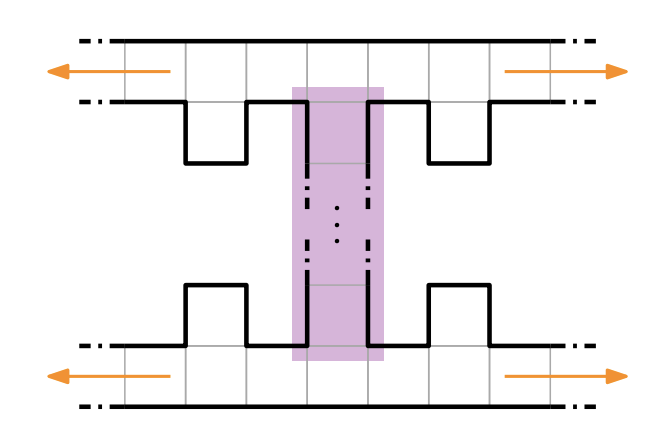
\includegraphics[width=0.5\textwidth]{images/dispersion_distance_3.png}
        \caption{Polyomino with dispersion distance at most 3}
        \label{fig:dispersion_distance_3}
    \end{figure}
\end{itemize}
\vspace{-0.8cm}
\subsubsection*{Scope of further research}
\vspace{-0.3cm}
\begin{itemize}
    \itemsep-0.3em
    \item It would be interesting to see if the problem is $NP$-complete for values of $l$ other than 5.
    \item It would be interesting to see how the problem changes with different types of polygons.
\end{itemize}

\printbibliography
\end{document}
